\chapter{Heavy Ion Collisions: A Primer} % Main chapter title

%----------------------------------------------------------------------------------------
\section{Measurable Quantities}
Due to the complexity inherent in colliding large nuclei containing a large number of nucleons (for instance 197 nucleons in Au) there is a multitude of metrics we can use to quantify the collision and the evolution of what happens after. For clarification, when talking about high energy physics analyses we refer to all data gathered from a single collision of two nucleons as an \textit{event}. The location where the collision takes place is called the \textit{event vertex} or often in collaboration literature since the z-axis is along the beam axis, the \textit{z vertex}. The high luminosity of heavy ion collisions (437 $nb^{-1}$ in 9 weeks for the data used in this analysis: Run 8 d+Au), produces a plethora of particles. As these particles travel from the event vertex through the various layers of detectors under the influence of the PHENIX magnetic field it leaves its own signature on each detector it passes through. These signatures for each given particle can be matched to form a trajectory from the event vertex through PHENIX. The set of data corresponding to location, kinematic, and detector specific variables (i.e. charge deposited, clusters fired, Cherenkov photons, etc) is called a \textit{track}. The determination of these variables is the topic of this chapter.

\section{Event Characterization}
When describing a heavy ion collision it is useful to introduce quantities that describe the initial conditions of the interacting nucleons. The set of variables that correspond to these conditions are called the \textit{event} or \textit{global} variables. They are used to accurately locate where the event took place inside the detector and the geometric configuration of the nuclei at the time of collision. These event variables are reconstructed largely by the extremely forward detectors: the \textit{Beam-Beam Counters} (BBC) and the \textit{Zero Degree Calorimeters}. 

\subsection{Centrality}
One such variable is \textit{centrality} and is used to describe how "head-on" two ions collide, that is, do they collide with complete cross sectional overlap or do they just barely glance each other. It is useful to quantify this overlap with a quantity called the \textit{impact parameter}, \textbf{b}. We define this impact parameter by measuring the distance between ion centers as depicted on the left-hand side of figure \ref{fig:cernfireball}. Note that the ions in this illustration appear squished in the x axis due to Lorentz contraction. Therefore, small impact parameters correspond to large ion-ion overlap in the collision and large impact parameters refer to glancing collisions. In heavy ion physics we call collisions with small impact parameters \textit{central collisions} and those with large impact parameters \textit{peripheral collisions}. Experimentally it is impossible to measure the distance between the two ion centers. In practice, centrality can also be quantified by the number of \textit{participants}, or the number of nucleons that collide/interact with each other, versus the number of \textit{spectators}, or the number of nucleons that do not collide. Since we know the number of total nucleons in each ion we can determine the number of participants by counting the number of spectators and subtracting them from the total number of nucleons. Colliding nucleons will produce particles in all directions however spectating nucleons will continue to travel down the beam pipe. We therefore can count the number of spectators by placing detectors at very high rapidity.

\begin{figure}[htbp!]
  \centering
    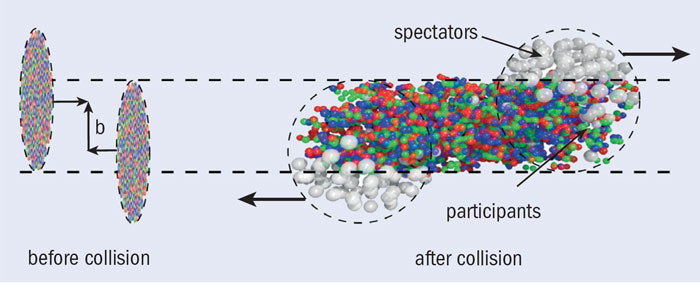
\includegraphics[width=1\textwidth]{Figures/spectatorsvsparticipants.jpg}
    \rule{35em}{0.5pt}
  \caption[Spectators and participant nucleons in a heavy ion collision]{Spectators and participant nucleons in a heavy ion collision \citep{cernhifireball}}
  \label{fig:cernfireball}
\end{figure}

Extending the terminology from impact parameters, we then define a collision with a large number of participants to be a \textit{central} collision and a collision with a small number of participants: a \textit{peripheral} collision. These are quantified in percents, 0$\%$ being most central collisions i.e. highest number of participants, $b=0$, two colliding ions overlap completely, and 100$\%$: ions completely miss each other, i.e. there are no participants, $b > R_{nucleus}$. Since ions are spherical in shape, centrality can be used as a way of describing the geometry of the collision region, central collisions have a more circular shape whereas peripheral collisions have a more almond-like shape.

\begin{figure}[htbp!]
  \centering
  \begin{subfigure}[b]{0.8\textwidth}
    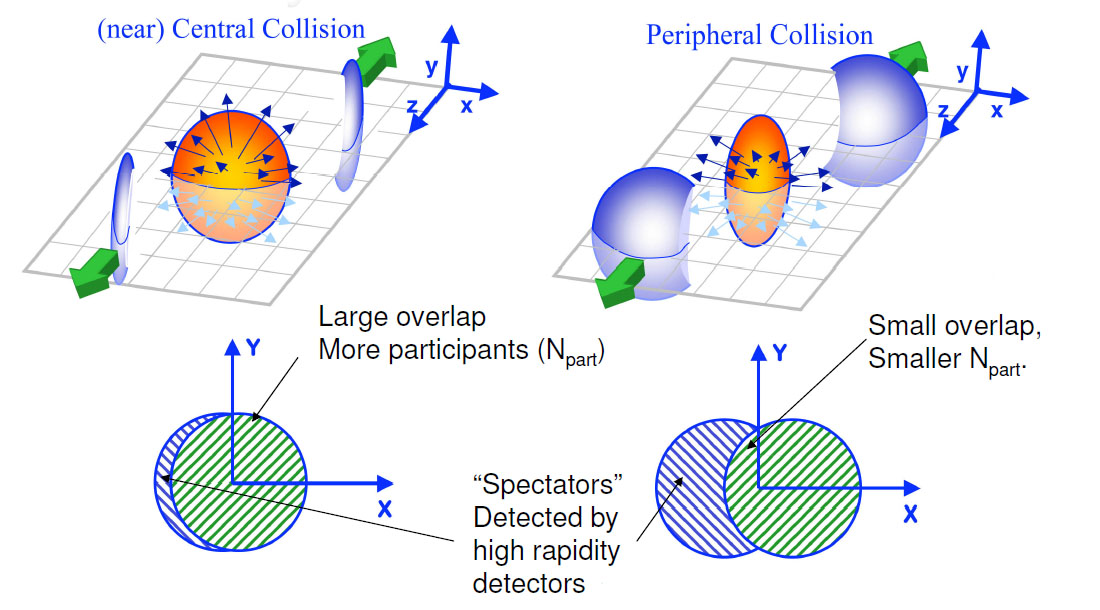
\includegraphics[width=0.5\textwidth]{Figures/centralvsperipheral.jpg}
    \end{subfigure}
    \begin{subfigure}[b]{0.8\textwidth}
    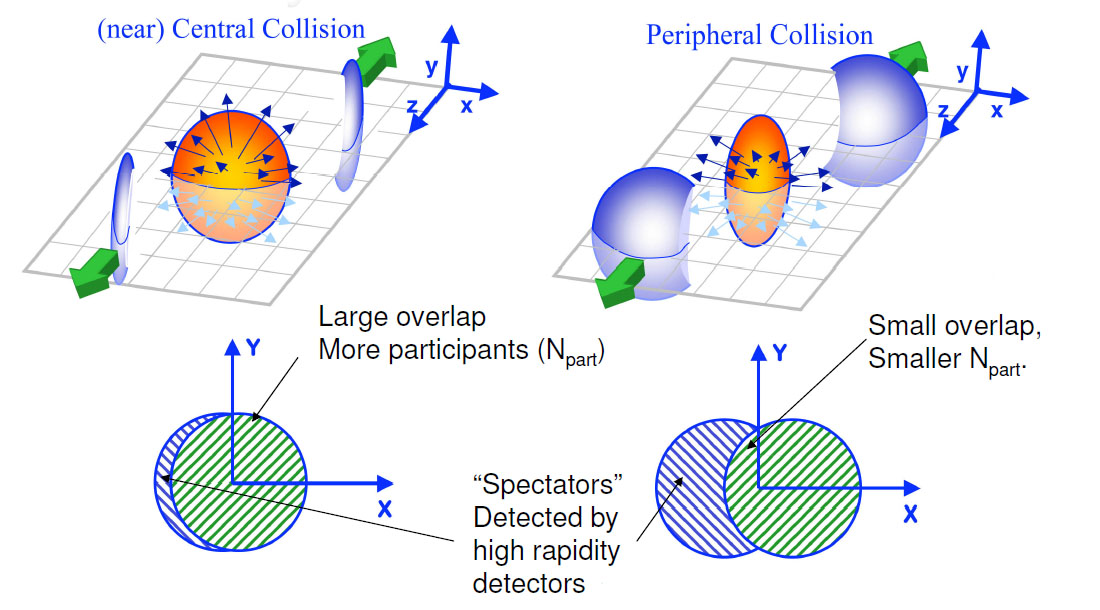
\includegraphics[width=0.5\textwidth]{Figures/centralvsperipheral.jpg}
    \end{subfigure}
    \rule{35em}{0.5pt}
  \caption[Central versus peripheral ion collisions]{Spectators and participant nucleons in a heavy ion collisions.}
  \label{fig:centralvsperipheral}
\end{figure}

\subsection{Event Vertex and Timing}
The event vertex is the location along the beam axis where the collision happened relative to the equidistant point between the two beam beam counters. That is, an event vertex value of 0 would be exactly in the center of the PHENIX detector, at equal distance from both BBCs. When a collision happens, the non colliding nucleons (spectators) continue to travel through the interaction region and are detected on the other side by the two BBCs. The time at which each cluster of spectators hits an individual BBC is measured. These two times, $T_1$ and $T_2$ respectively, can be used to calculate both the event vertex ($z_{vtx}$) and the initial time the collision takes place ($T_0$) as follows\citep{Mitchell:2002wu}:

\begin{equation}
 z_{vtx} = \frac{T_1 - T_2}{2c} \qquad\text{and}\qquad T_0 = \frac{T_1 + T_2}{2}
\end{equation}

This initial time is used to start the stopwatch of the event and is used in conjunction with other detectors to to find the time a produced particle takes to travel from the vertex to a detector.

\begin{figure}[htbp!]
  \centering
    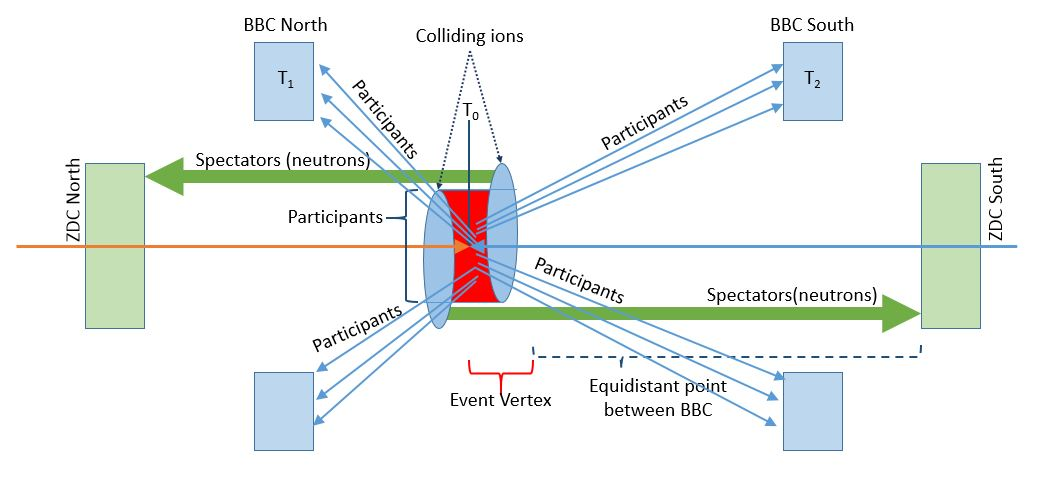
\includegraphics[width=1\textwidth]{Figures/BBCevtchar.JPG}
    \rule{35em}{0.5pt}
  \caption[Diagram of BBC event characterization]{Diagram of BBC event characterization}
  \label{fig:bbcvtx}
\end{figure}

\section{Track Reconstruction}

\subsection{Variables for Track Selection}
After the collision, particles fly outward from the vertex under the various mechanisms that take place within the formation and evolution of the QGP. Due to the high multiplicity of tracks resulting from a heavy ion collision and the various complexities that arise when using a multifaceted complicated detector system to reconstruct track trajectories, it is important to come up with a metric by which to measure the quality of the tracks in order to discern which tracks are able to be reconstructed cleanly versus those which, for whatever anomalous reasons, would not be advantageous to analyze.

The process of determining the track trajectory through the PHENIX detector is called \textit{track matching} and it utilizes the various layers of the Drift Chamber and Pad Chambers in concert to determine track momentum due to the varying curvature of tracks of different momenta traveling through a magnetic field. Tracks are reconstructed in the DC and PC1 using an algorithm called a combinatorial Hough Transform which works very well for particles whos $p_T$ is $>$200 MeV/c \citep{Mitchell:2002wu}. 
track quality

\subsection{Particle Identification}
Using the TOF detectors' high resolution timing measurements I am able to identify particles which have long lifetime relative to the event duration i.e. particles whose lifetimes are long enough such that they do not decay before leaving the detector. For this analysis, these particles of interest are the charged pions ($\pi^{\pm}$), charged kaons ($k^{\pm}$), and protons/antiprotons ($p/\bar{p}$). Since the masses of these particles are distinct, plotting the momentum vs time of flight can show clear separation between pion, kaon, and proton signals (see fig \ref{fig:tofchargemom}). 

\begin{figure}[htbp!]
  \centering
    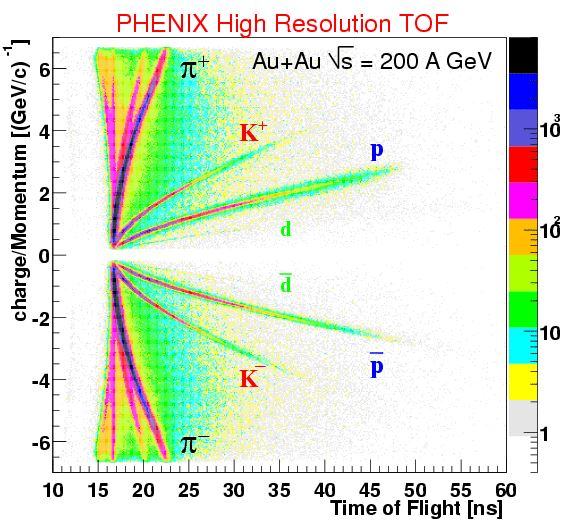
\includegraphics[width=0.7\textwidth]{Figures/tofchargemom.JPG}
    \rule{35em}{0.5pt}
  \caption[Particle separation in the TOF]{Particle separation in the TOF \citep{tofchargemom}}
  \label{fig:tofchargemom}
\end{figure}

While visually the individual particle signatures are easily identifiable, computationally it is advantageous to convert units so that the signatures only depend on a single variable. After the collision, the QGP fireball is expanding rapidly however the constituent outgoing tracks traversing the distance scales in the detector do not experience appreciable deceleration. We know from basic kinematics that we can calculate the velocity, v, of an object traveling at a constant speed:

\begin{equation}
v=\frac{L}{t} \implies t=\frac{L}{v},
\end{equation}
where t is the time it takes to travel some path length, L. It is useful to define the relative speed of the particle compared to the speed of light, c, as $\beta = v/c$ and substitute it in for v. We also know from the relativistic identities that $\beta = p/E$ and $E^{2} = p^{2} + m^{2}$. The equation is then: 

\begin{equation}
t=\frac{L}{v} = t=\frac{L}{c\beta} = \frac{L}{c} \frac{E}{p} = \frac{L}{c} \frac{\sqrt{p^{2} + m^{2}}}{p}.
\end{equation}

which can be solved for $m^{2}$ to give the mass vs time relation:

\begin{equation}
m^{2} = p^{2} \bigg\{ \frac{t^{2}}{L^{2}} -1 \bigg\}.
\end{equation}

Note that since the distance from the event vertex to the detector is constant and for that distance scale the velocity, and therefore also the momentum, can be treated as constant, $m^{2}$ depends on two constant terms if we take measurements in bins of p. Since we are talking about radially outward traveling tracks, this p is, in practice, $p_{T}$. Therefore if we do arithmetic on the track variables we are able to plot $m^{2}$ vs $p_{T}$ which gives us a much easier to analyze representation of the individual particle signatures.

\begin{figure}[htbp!]
  \centering
    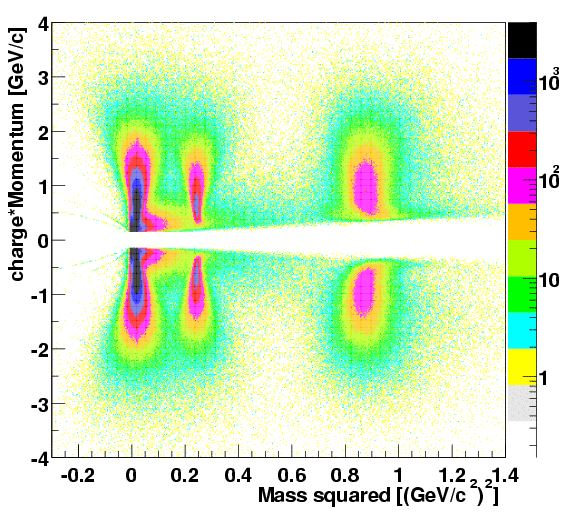
\includegraphics[width=0.7\textwidth]{Figures/m2tofvspt.jpg}
    \rule{35em}{0.5pt}
  \caption[$m^{2}$ vs $p_{T}$ showing clear constant separation of particle signatures.]{$m^{2}$ vs $p_{T}$ showing clear constant separation of particle signatures. \citep{tofchargemom}}
  \label{fig:m2tofvspt}
\end{figure}

\pagebreak
\pagebreak
